\documentclass[11pt, a4paper]{article}

\usepackage{tikz}
\usepackage{graphicx}
\usepackage{amsfonts}
\usepackage{appendix}
\usepackage[utf8]{inputenc}
\usepackage[english]{babel}

\date{}
\title{Exoplanets detection using random forest}
\author{Lorenzo Loconte}

\begin{document}

\maketitle
\begin{abstract}
  This work consists of identifying exoplanets using random forest which hyperparameters are automatically optimized with techniques that come from the \texttt{AutoML} research.
  The model is trained using the processed data that comes from the \texttt{NASA Kepler} project of discovering exoplanets (i.e. planets outside our solar system).
  The hyperparameters of the model are optimized and cross-validated with \texttt{Hyperband}, a simple yet effective and scalable method for hyperparameters optimization.
  The dataset used in this work can be found at \textbf{https://exoplanetarchive.ipac.caltech.edu}.
\end{abstract}

\section{Introduction}
  \paragraph{Kepler Object of Interest}
    The dataset used in this work is the cumulative list of the \texttt{Kepler Object of Interest} (\texttt{KOI}) that comes from the \texttt{NASA Kepler} project of discovering exoplanets.
    The dataset is composed by a list of examples regarding exoplanets. Each example have a label indicating if the corresponding exoplanet is candidate, false positive or confirmed. The provided dataset consists of a lot of heterogeneous features. For the classification task the selected features can be found in Appendix \ref{appendix:features}. The candidate exoplanets (i.e. the exoplanets which existence is uncertain) are discarded in order to reduce noise and improve the learning process.
    For simplicity all the examples having null values are removed from the dataset. Furthermore, all the selected features are numeric and so the preprocessing method applied to the dataset is the standard normalization.
    The resulting dataset contains \texttt{6884} samples, which \textasciitilde \texttt{67\%} are false positives and the remaining are confirmed.
    
  \paragraph{Random Forests}
    The model used for the classification task is a random forest, an ensemble of random decision trees. The prediction of the random forest is computed as the mode of each tree's classification. Random decision forests correct the habit of decision trees of overfitting. Each tree of the forest is trained on a subset of the features and samples. The hyperparameters of the random forest are optimized and cross-validated using approaches that come from the \texttt{AutoML} research. The following hyperparameters are optimized:
    \begin{itemize}
      \item The split criterion (Gini impurity or information gain, see Appendix \ref{appendix:splitcriterions} for details)
      \item The maximum depth of each tree
      \item The minimum number of samples required to split an internal node
      \item The minimum number of samples to be at a leaf node
      \item The percentage of features to use for each tree
    \end{itemize}
  As the next section will expose, the number of trees in the random forest is not considered an hyperparameter because it represents the budget of the hyperparameters optimization algorithm chosen. In this work we refer with budget as the computational cost of training and cross-validating a certain model.

\section{Hyperparameters Tuning}
  The hyperparameters optimization task consists to find the hyperparameters for a model that maximize a certain score. In this work we refer to hyperparameters as the ones that cannot be trained (e.g. the ones described in the previous section).
  There are a lot of different techniques for hyperaparameters optimization, some of them are the following:
  \begin{itemize}
    \item Random Search
    \item Grid Search
    \item Hyperband
    \item Bayesian Optimization
    \item Hybrid Approaches (like \texttt{BOHB})
  \end{itemize}
  In this work, given the restricted hyperparameters search space, we used \textit{Hyperband} as the hyperparameters optimization algorithm. It's a simple method that consists of random sampling some points in the hyperparameters space and cross-validating them on the validation set. After that we extract a portion of the best hyperparameters and build more complex random forests. After some iterations we pick the best hyperparameters point corresponding to the best model.
  Even if it is a simple algorithm, it is well scalable on multiple CPUs because we assume that every point in the hyperparameters space is independent from the others.
  In this work the hyperparameters search space can be defined formally as:
  \[\Omega = \{gini, entropy\} \times \mathbb{N}^{3} \times (0, 1]\]
  Table \ref{table:hyperparameters} shows the subset of the search space used in this work.

  \begin{table}
    \centering
    \begin{tabular}{|c c|}
      \hline
      Hyperparameters & Values \\
      \hline\hline
      Split Criterions & $\{gini, entropy\}$ \\
      \hline
      Maximum Depth & $\{8,9,...,32\}$ \\
      \hline
      Minimum samples to split & $\{2,3,...,16\}$ \\
      \hline
      Minimum samples at a leaf & $\{1,2,...,10\}$ \\
      \hline
      Features percentage & $(0, 1]$ \\
      \hline
    \end{tabular}
    \caption{The hyperparameters space subset used in this work.}
    \label{table:hyperparameters}
  \end{table}

  The optimization task consists to find a point in the hyperparameters space:
  \[\omega=(c, h, k, t, p)\in\Omega\]
  where $c$ is the split criterion, $h$ is the maximum depth, $k$ is the minimum number of samples to split, $t$ is the minimum number of samples at a leaf, $p$ is the features percentage for each tree, such that the random forest built from these hyperparameters maximize a certain score. The choice of this score is dependent from the task. For simplicity we use the $F_{1}$ score (i.e. we want to maximize both \textit{Precision} and \textit{Recall}).

\section{Conclusion and Results}
  As you can see from Table \ref{table:confusion} the false positives count (the number of examples, which are predicted as exoplanets, but that are not) and the false negatives count (the number of actual exoplanets not being discovered), are pretty low.

  As you can see from Table \ref{table:benchmark} the auto-tuned random forest used in this work obtained a way better precision and recall. For this task we want to have a better recall because we want to maximize the number of actual exoplanets discovered.
  In the end we present Table \ref{table:importances} that shows the importances of the first five out eighteen features used.
  
  \begin{table}
    \centering
    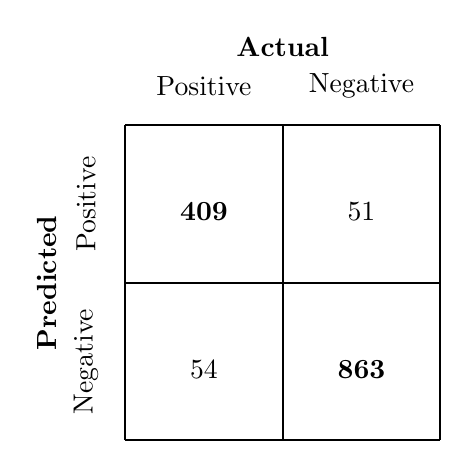
\begin{tikzpicture}[scale=2]
      % Draw the box
      \draw[thick] (0, 0) -- (2, 0);
      \draw[thick] (0, 0) -- (0, 2);
      \draw[thick] (2, 2) -- (2, 0);
      \draw[thick] (2, 2) -- (0, 2);
      \draw[thick] (0, 1) -- (2, 1);
      \draw[thick] (1, 0) -- (1, 2);
      % Draw the headers
      \node[rotate=0] (h1) at (1, 2.5) {\textbf{Actual}};
        \node[rotate=0] (h11) at (0.5, 2.25) {Positive};
        \node[rotate=0] (h12) at (1.5, 2.25) {Negative};
      \node[rotate=90] (h2) at (-0.5, 1) {\textbf{Predicted}};
        \node[rotate=90] (h21) at (-0.25, 1.5) {Positive};
        \node[rotate=90] (h22) at (-0.25, 0.5) {Negative};
      % Draw the category values
      \coordinate[label={\textbf{409}}] (PP) at (0.5, 1.33);
      \coordinate[label={ 54}] (NP) at (0.5, 0.33);
      \coordinate[label={ 51}] (PN) at (1.5, 1.33);
      \coordinate[label={\textbf{863}}] (NN) at (1.5, 0.33);
    \end{tikzpicture}
    \caption{Confusion matrix over the test set.}
    \label{table:confusion}
  \end{table}

  \begin{table}
    \centering
    \begin{tabular}{|c c c c|}
      \hline
      Model & Precision & Recall & $F_{1}$  \\
      \hline\hline
      k-NN & 0.922 & 0.829 & 0.873 \\
      \hline
      SVC & 0.925 & 0.875 & 0.899 \\
      \hline
      2-layer NN & 0.930 & 0.917 & 0.926 \\
      \hline
      Random Forest & 0.938 & 0.932 & 0.938 \\
      \hline
      \textbf{Random Forest w/\texttt{Hyperband}} & \textbf{0.944} & \textbf{0.941} & \textbf{0.943} \\
      \hline
    \end{tabular}
    \caption{Precision, recall and $F_{1}$ metrics of several models for comparison. The hyperparameters were optimized automatically. In this table it was built with the following hyperparameters found: $\omega = (entropy, 32, 7, 2, 0.5)$}
    \label{table:benchmark}
  \end{table}

  \begin{table}
    \centering
    \begin{tabular}{|c c c|}
    \hline
    Feature \# & Description & Importance \\
    \hline\hline
    7 & Planetary Radius & 0.196 \\
    5 & Planet-Star Radius Ratio & 0.118 \\
    6 & Fitted Stellar Density & 0.078 \\
    1 & Orbital Period & 0.075 \\
    8 & Orbit Semi-Major Axis & 0.071 \\
    \hline
    \end{tabular}
    \caption{Features importances in descending order.}
    \label{table:importances}
  \end{table}

\newpage
\begin{appendix}
  \section{Split criterions}
    \label{appendix:splitcriterions}
    \subsection{Gini impurity}
      Citing \texttt{wikipedia.org}, Gini impurity is a measure of how often a randomly chosen element from the set would be incorrectly labeled if it was randomly labeled according to the distribution of labels in the subset. To compute Gini impurity for a set of items with $J$ classes, suppose $i\in\{1,2,...,J\}$, and let $p_{i}$ be the faction of items labeled with class $i$ in the set.
      \[{I} _{G}(p)=\sum _{i=1}^{J}p_{i}\sum _{k\neq i}p_{k}=\sum _{i=1}^{J}p_{i}(1-p_{i})=\sum _{i=1}^{J}p_{i}-\sum _{i=1}^{J}{p_{i}}^{2}=1-\sum _{i=1}^{J}{p_{i}}^{2}\]
    \subsection{Information gain}
      Information gain is based on the concept of entropy and information content from information theory. For each node of the tree, the information value represents the expected amount of information that would be needed to specify whether a new instance should be classified yes or no, given the example reached that node. Suppose $i\in\{1,2,...,J\}$, where $J$ is the number of classes, and let $p_{i}$ be the faction of items labeled with class $i$ in the set.
      \[IG(T, a)=\mathrm{H}(T)-\mathrm{H}(T|a)=-\sum _{i=1}^{J}p_{i}\log _{2}{p_{i}}-\sum _{a}{p(a)\sum _{i=1}^{J}-\mathrm{P}(i|a)\log _{2}{\mathrm{P}(i|a)}}\]
      where $T$ is a set of training examples, $\mathrm{H}(T)$ is the entropy of $T$ and $\mathrm{H}(T|a)$ is the conditional entropy for $T$ given the feature $a$.

  \section{Exoplanet Features}
    \begin{enumerate}
      \item Orbital Period [days]
      \item Impact Parameter
      \item Transit Duration [hrs]
      \item Transit Depth [ppm]
      \item Planet-Star Radius Ratio
      \item Fitted Stellar Density [g/cm**3]
      \item Planetary Radius [Earth radii]
      \item Orbit Semi-Major Axis [AU]
      \item Inclination [deg]
      \item Equilibrium Temperature [K]
      \item Insolation Flux [Earth flux]
      \item Stellar Effective Temperature [K]
      \item Stellar Surface Gravity [log10(cm/s**2)]
      \item Stellar Radius [Solar radii]
      \item Stellar Mass [Solar mass]
      \item RA [decimal degrees]
      \item Dec [decimal degrees]
      \item Kepler-band [mag]
    \end{enumerate}
    \label{appendix:features}
\end{appendix}

\end{document}
